Fungsi (Function) adalah sekumpulan program yang diberi nama, sehingga
dengan demikian jika program itu diperlukan dapat dipanggil kembali.
Walaupun Pemrograman Berorientasi Objek telah menggeser perhatian dari
fungsi ini, namun fungsi tetap saja merupakan bagian paling inti dalam
suatu program. Fungsi global bisa berada di luar kelas maupun objek.

Fungsi dapat melakukan manipulasi terhadap data dan dapat mengembalikan
suatu nilai. Semua program yang ditulis dengan bahasa C++ paling tidak
mempunyai sebuah fungsi, yaitu \texttt{main()}, fungsi ini akan
dipanggil secara otomatis ketika program dieksekusi, sedangkan fungsi
yang lain baru akan bekerja ketia fungsi tersebut dipanggil. Karena
fungsi ini bukan merupakan bagian dari objek, maka fungsi ini dipanggil
secara global, dapat diakses dari manapun dalam program yang ditulis

Setiap fungsi diberi nama, dan ketika dalam suatu program dijumpai nama
tersebut, maka eksekusi program akan dialihkan ke tubuh (isi) fungsi
tersebut, setelah selesai, yaitu ditandai dengan statemen
\texttt{return} atau tanda kurung kurawal tutup, maka akan kembali ke
progam utama melanjutkan ke baris program berikutnya. Peristiwa ini
dinamakan pemanggilan fungsi, berikut ini adalah ilustrasi mengenai
pemanggilan fugsi :

\begin{figure}[htbp]
\centering
\includegraphics[width=0.8\textwidth]{images/capture4-1.png}
\caption{Ilustrasi penanganan fungsi}
\end{figure}

Fungsi yang baik mengerjakan sebuah pekerjaan yang spesifik, mudah
dipahami dan mudah dikenali berdasarkan nama fungsi tersebut. Pekerjaan
yang kompleks seharusnya dipecah-pecah menjadi beberapa fungsi yang
nantinya dapat dipanggil ketika diperlukan.

Fungsi terdiri dari 2 macam, yaitu fungsi yang dibuat sendiri
(\emph{user-defined}) dan fungsi standard (\emph{built-in}).Fungsi
standard merupakan bagian dari paket kompiler yang kita pakai yang sudah
tersedia untuk digunakan, sedangkan fungsi yang dibuat sendiri adalah
fungsi yang kita tulis sebelum dapat dipergunakan.

\section{Konsep Dasar Fungsi}\label{konsep-dasar-fungsi}

Fungsi sebenarnya mirip dengan prosedur (pada bhs. Pascal), dan kedua
hal ini disebut sebagai \texttt{Subrutin}. Kedua jenis subrutin ini
(fungsi dan prosedur) memiliki kegunaan yang sama, yaitu melakukan tugas
tertentu. Perbedaannya fungsi selalu mengembalikan suatu nilai setelah
dipanggil sedangkan prosedur tidak.

Kita memerlukan subrutin, karena dalam program yang besar akan lebih
baik jika tugas tertentu dilakukan oleh subrutin tertentu, dengan
demikian program akan menjadi lebih mudah dibaca dan dipelihara.
\begin{quotation}
	\textbf{Catatan :}
	
	Fungsi bisa dikatakan sebagai bentuk
	lain dari instruksi yang dapat memberikan sebuah nilai apabila diberi
	masukan yang dibutuhkan. Masukan tersebut dikenal dengan istiah
	Parameter.
\end{quotation}
 

Fungsi-fungsi merupakan elemen utama dari program bahasa C++. Program
dari bahasa C++ dibentuk dari kumpulan fungsi, mulai dari fungsi utama
dengan nama \texttt{main()}, fungsi-fungsi pustaka (standar) dan
fungsi-fungsi yang dibuat sendiri oleh pemrogram (UDF = \emph{User
Defined Function}). Fungsi-fungsi banyak digunakan dengan dua alasan
utama, yaitu:

\begin{enumerate}
\def\labelenumi{\arabic{enumi}.}
\item
  Fungsi-fungsi menjadikan program C++ mempunyai struktur yang jelas.
  Dengan memisahkan langkah--langkah detail ke satu atau lebih
  fungsi--fungsi, maka fungsi utama (\texttt{main()}) akan menjadi lebih
  pendek, jelas dan mudah dimengerti. Hal seperti ini menunjukan suatu
  struktur program yang baik.
\item
  Fungsi-fungsi dapat digunakan untuk menghindari penulisan program yang
  sama ditulis secara berulang-ulang. Selanjutnya bagian program yang
  membutuhkan langkah-langkah yang sama tidak perlu selalu dituliskan,
  melainkan cukup memanggil fungsi-fungsi tersebut.
\end{enumerate}

Suatu fungsi harus diberi nama supaya dapat dipanggil dari bagian
program yang membutuhkannya. Tugas yang dilakukan oleh suatu fungsi
dapat berupa tugas input/output, penyeleksian atau tugas-tugas
perhitungan dan sebagainya.

\section{Mendefinisikan Fungsi}\label{mendefinisikan-fungsi}

Secara umum, fungsi terdiri dari dua komponen yaitu definisi fungsi dan
tubuh fungsi. Isi dari definisi fungsi adalah : tipe dari fungsi, nama
dari suatu fungsi dan paramter-parameter yang digunakan. Tubuh dari
fungsi berisikan statemen-statemen yang akan melakukan tugas yang
diberikan oleh fungsi tersebut. Tubuh suatu fungsi diawali dengan tanda
kurung kurawal buka dan diakhiri dengan tanda kurung kurawal tutup.
Beikut ini adalah bentuk umum dari suatu fungsi:

\begin{lstlisting}[language=c++, numbers=none]
<tipe> <nama_fungsi>([<paramter1>, <paramter2> ,...])
{
<tubuh fungsi>
[return <ekspresi>]
}
\end{lstlisting}

Definisi fungsi ditulis sebelum dituliskan tubuh fungsi dan tidak
diakhiri dengan tanda titik koma. Tipe dari definisi fungsi sesuai
dengan tipe data dari nilai yang dikembalikan jika fungsi itu mempunyai
statment \texttt{return}, jika tidak terdapat statement \texttt{return}
tipe ini diberi tipe \texttt{void}. Nama suatu fungsi dibentuk sendiri
oleh pemrogram sesuai dengan syarat penamaan identifier yang telah
dibahas pada bab 2 dan nama fungsi yang baik mencerminkan pekerjaan dari
fungsi tersebut. Parameter suatu fungsi dapat dituliskan dengan
dipisahkan oleh tanda koma, bisa mempunyai beberapa parameter namun
dapat juga tidak mempunyai parameter sama sekali. Parameter dibutuhkan
jika dalam tubuh fungsi memerlukan nilai dari luar fungsi. Parameter ini
dinamakan parameter formal. Berikut ini adalah contoh cara
mendefinisikan fungsi.

\begin{lstlisting}[language=c++, numbers=none]
int terbesar(int bil1, int bil2)
{
int hasil;
if (bil1>bil2)
kembali = bil1;
else
kembali = bil2;
return kembali;
}
\end{lstlisting}

\section{Deklarasi Fungsi
(Prototype)}\label{deklarasi-fungsi-prototype}

Suatu fungsi harus dideklarasikan sebelum digunakan, jika suatu fungsi
tidak dideklarasikan maka fungsi tersebut tidak akan bisa dipanggil.
Deklarasi tersebut akan memberitahukan kepada kompiler mengenai nama
fungsi, tipe data kembalian dan parameter dari fungsi, sedangkan
definisi dari fungsi memberitahukan kepada kompiler mengenai cara kerja
fungsi. Deklarasi fungsi ini dinamakan prototipe (\emph{prototype}).

Ada tiga cara mendeklarasikan fungsi (membuat \emph{prototype}), yaitu :

\begin{itemize}
\tightlist
\item
  Menuliskan prototipe ke dalam sebuah file, kemudian menggunakan
  directive \texttt{\#include} untuk menyertakannya.
\item
  Tuliskan prototype di dalam file yang memakai fungsi tersebut.
\item
  Definisikan fungsi di file yang memakai fungsi tersebut di posisi
  sebelum pemanggilnya, dengan demikian definisi fungsi ini bertidak
  sebagai prototype itu sendiri.
\end{itemize}

Meskipun kita dapat mendefiniskan fungsi sebelum digunakan, sehingga
bisa menghindari pembuatan prototype, namun cara ini merupakan cara yang
tidak baik karena tiga alasan. Pertama, menampilkan fungsi dalam sebuah
file dengan urutan tertentu adalah tidak baik, karena akan menyulitkan
ketika terjadi perubahan program.

Kedua, ada kemungkinan fungsi pertama memerlukan pemanggilan fungsi
kedua, tetapi ada juga kemungkinan fungsi kedua memanggil fungsi yang
pertama. Pada kasus semacam ini tidak mungkin menempatkan definisi
fungsi pada urutan yang benar tanpa membuat prototype.

Ketiga, penggunaan prototype merupakan teknik penelusuran kesalahan yang
baik dan handal. Ketika suatu prototype mendeklarasikan fungsi dengan
parameter tertentu dan nilai kembalian tertentu, maka kompiler akan
menjaga konsistensinya dengan definisi fungsi tanpa harus menunggu
program dijalankan.

Compiler C++ dapat memeriksa tipe data melalui parameter-parameter
(actual parameter) yang dikirimkan dari program yang menggunakannya,
dengan terlebih dahulu menyebutkan prototype fungsi tersebut. Jika
terjadi kesalahan perbedaan antara tipe-tipe data parameter nyata yang
dikirim dengan tipe-tipe data parameter formalnya, maka dapat diketahui
melalui ketidakcocokan antara compiler untuk tipe data tersebut.

Prototype fungsi standard berada di file-file judulnya, dalam fungsi
pustaka sebagai contoh, fungsi pustaka \texttt{printf()}, prototypenya
berada di dalam file judul \texttt{stdio.h}. Pencantuman prototype
fungsi dapat menggunakan preprocessor directive \texttt{\#include}.

\subsubsection*{Contoh  Membuat Fungsi yang mengembalikan nilai.}

\begin{enumerate}
\def\labelenumi{\arabic{enumi}.}
\item
  Buka Qt Creator dan buat project Qt Console Application baru dengan
  nama Contoh \ref{membuat-fungsi-yang-mengembalikan-nilai}, kemudian tulis kode berikut.

\begin{lstlisting}[language=c++, caption=Membuat Fungsi yang mengembalikan nilai, label=membuat-fungsi-yang-mengembalikan-nilai]
#include <QtCore/QCoreApplication>
#include <iostream>
int absolut(int bil);
int main(int argc, char *argv[])
{
  using namespace std;
  QCoreApplication a(argc, argv);
  int bilangan = -10;
    cout << "Bilangan : " << bilangan << endl;
    cout << "Dimutlakkan menjadi : " << absolut(bilangan) << endl;
  return a.exec();
  }
  int absolut(int bil){
    if(bil<0)
    return - bil;
    else
    return bil;
}
\end{lstlisting}
\item
  Kemudian jalankan kode diatas dengan menekan tombol Ctrl + R, outputnya
  adalah sebagai berikut.
\end{enumerate}
\begin{lcverbatim}
Bilangan : -10
Dimutlakkan menjadi : 10
\end{lcverbatim}


\textbf{Analisa Program :}

\begin{itemize}
\tightlist
\item
  Pada program diatas baris ketiga tertulis :
  \texttt{int\ absolut(int\ bil);} inilah yang disebut sebagai
  prototype, ditulis sebelum fungsi yang memakainya, yaitu
  \texttt{main()}.\\
\item
  Pada tubuh pogram, terdapat pemanggilan fungsi :


\begin{lstlisting}[language=c++, numbers=none]
	cout << "Dimutlakkan menjadi : " << absolut(bilangan)
	<< endl;
\end{lstlisting}

Tampak pada hasil eksekusi bahwa nama fungsi tersebut digantikan dengan
nilai 10, yaitu nilai kembalian fungsi, ini menunjukkan bahwa fungsi
\texttt{absolut()}mengembalikan nilai.


\item
  Di bawah fungsi \texttt{main()} terdapat sebuah blok program dengan
  nama \texttt{absolut()}, inilah yang\\
  dinamakan definisi fungsi.

\end{itemize}
\begin{quotation}
		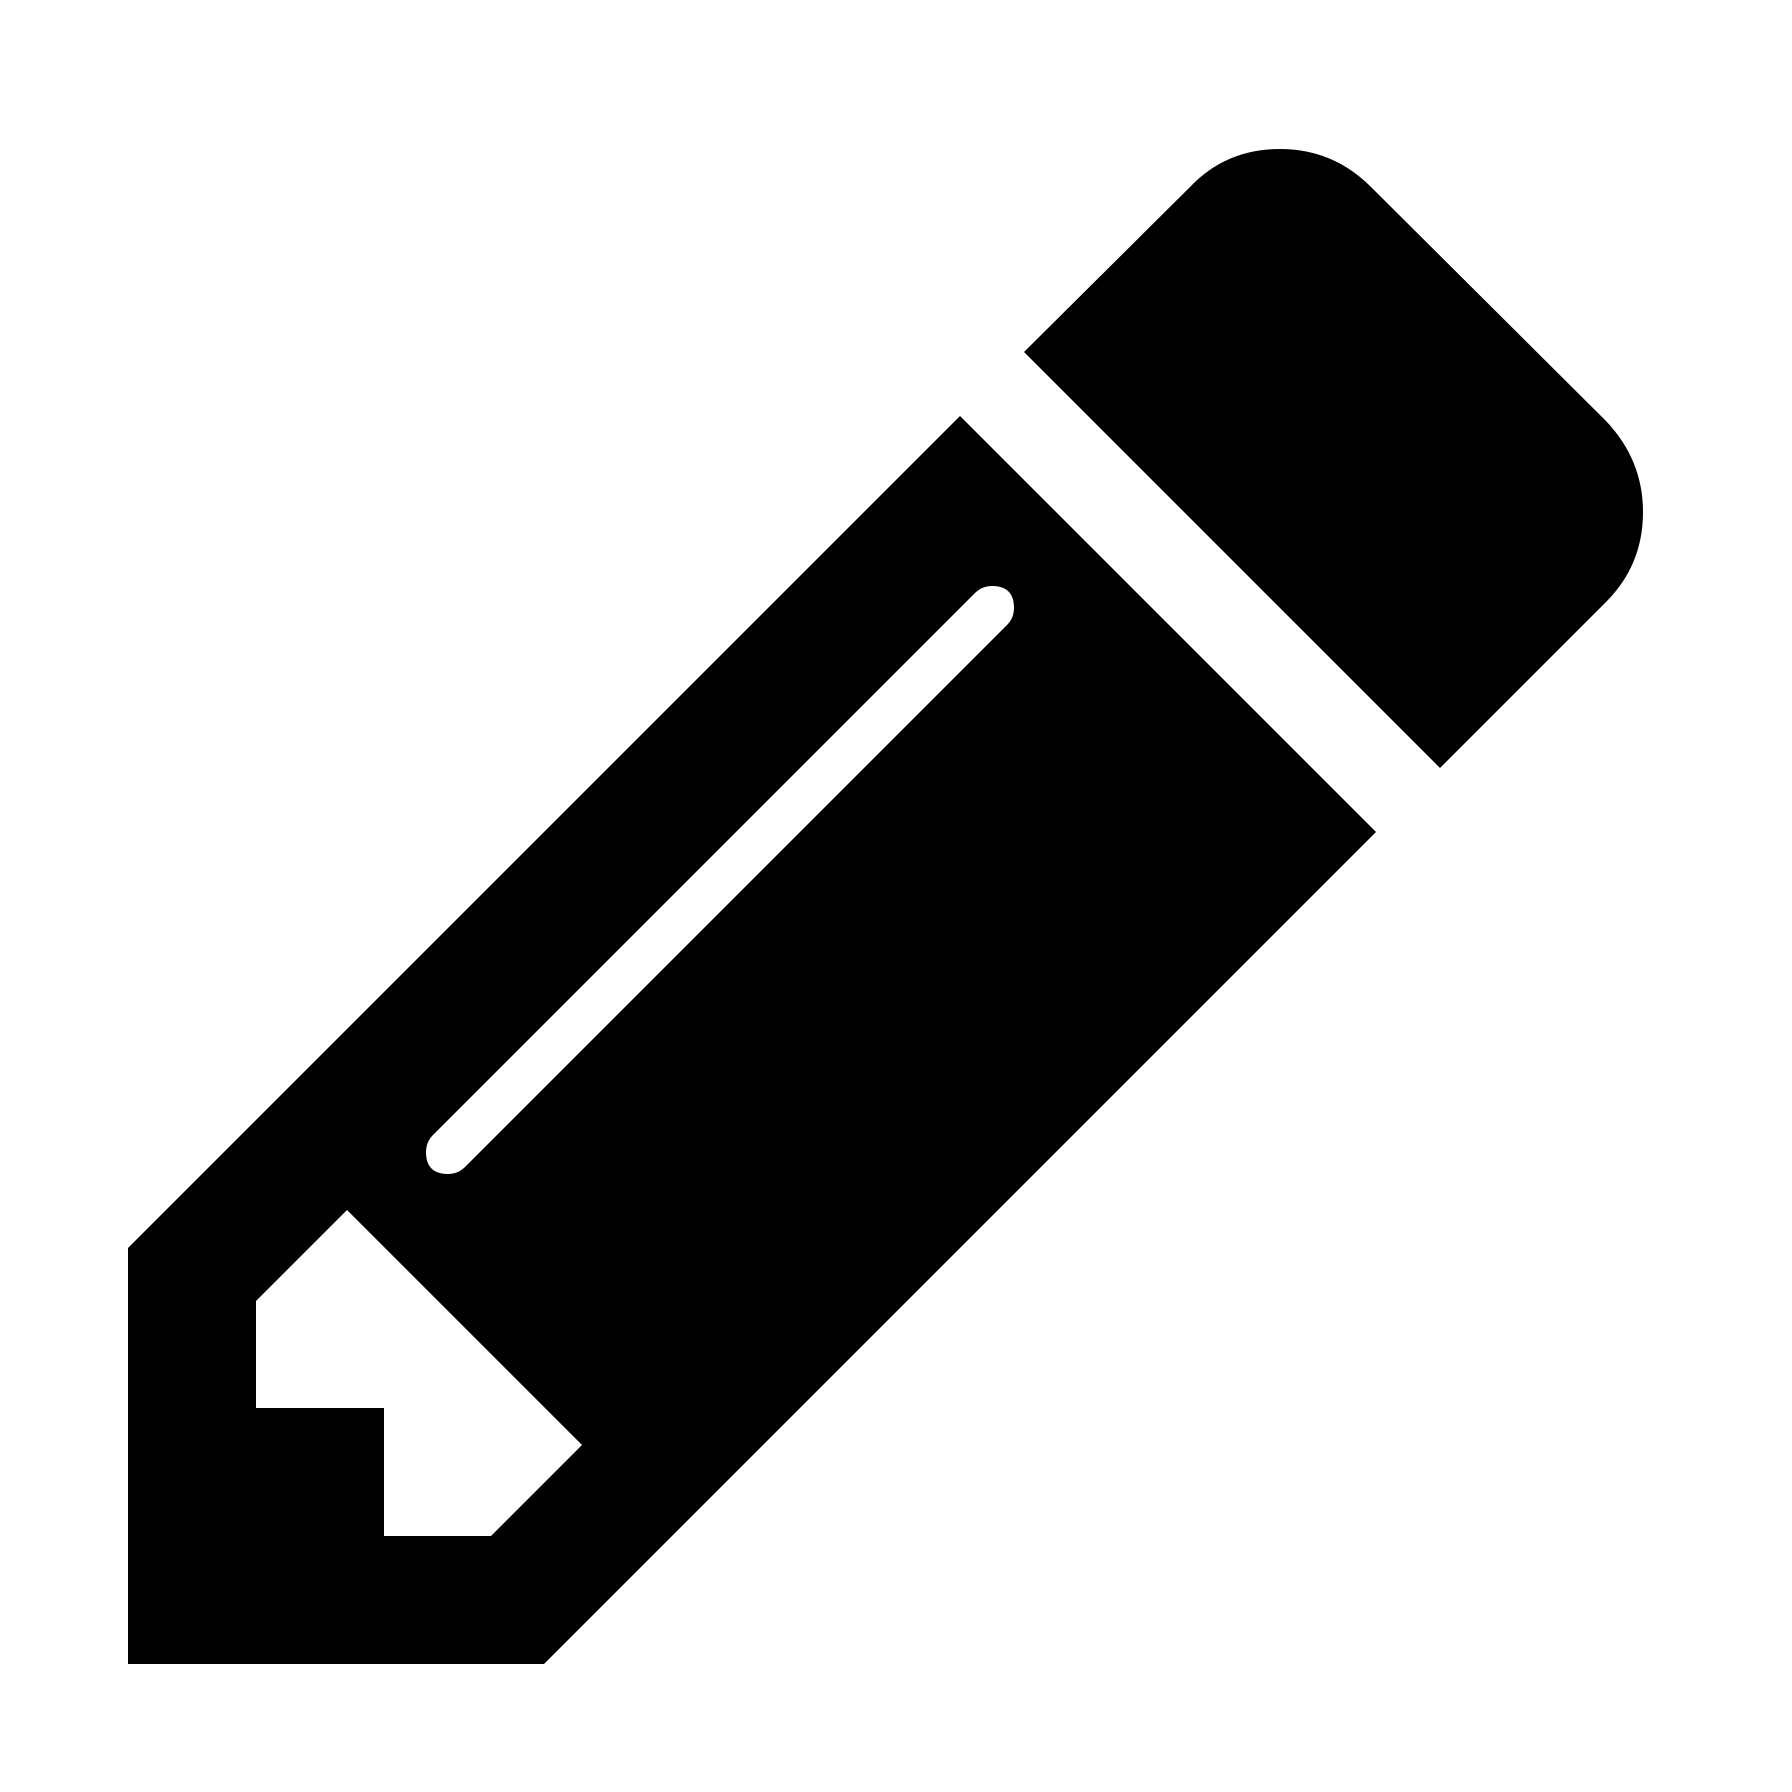
\includegraphics{images/pencil}	 \textbf{Catatan :}
		
		Nama parameter pada prototype tidak
		harus sama dengan nama parameter pada definisi fungsi, oleh karena itu
		prototype tersebut di atas boleh juga dituliskan seperti berikut :
		
		\begin{lstlisting}[language=c++, numbers=none]
		int absolut(int x);
		\end{lstlisting}
	
	 
\end{quotation}


\section{Hasil Balik Fungsi}\label{hasil-balik-fungsi}

Suatu fungsi dalam menyelesaikan tugasnya, dapat hanya melakukan suatu
tugas tanpa memberikan suatu nilai kembalian atau melakukan suatu tugas
yang kemudian memberikan suatu nilai kembalian. Fungsi yang hanya
menampilkan hasil di layar merupakan suatu fungsi yang hanya melakukan
tugasnya saja tanpa memberikan hasil balik. Untuk membuat fungsi yang
tidak mempunyai nilai kembalian digunakan tipe data void untuk tipe
fungsi tersebut dan pada tubuh definisi fungsi tidak ada satmenet
return.

\subsubsection*{Contoh  Membuat Fungsi yang tidak mengembalikan nilai.}

\begin{enumerate}
\def\labelenumi{\arabic{enumi}.}
\item
  Buka Qt Creator dan buat project Qt Console Application baru dengan
  nama contoh \ref{membuat-fungsi-yang-tidak-mengembalikan-nilai}, kemudian tulis kode berikut.

\begin{lstlisting}[language=c++, caption=Membuat Fungsi yang tidak mengembalikan nilai, label=membuat-fungsi-yang-tidak-mengembalikan-nilai]
#include <QtCore/QCoreApplication>
#include <iostream>
void hello(int kali);
int main(int argc, char *argv[])
{
QCoreApplication a(argc, argv);
hello(3);
return a.exec();
}
void hello(int kali){
using namespace std;
for(int x=0;x<kali;x++)
cout << "Hello World!" << endl;
}      
\end{lstlisting}
\item
  Kemudian jalankan kode diatas dengan menekan tombol Ctrl+R, outputnya
  adalah sebagai berikut.
\end{enumerate}
\begin{lcverbatim}
Hello World!
Hello World!
Hello World!
\end{lcverbatim}


\textbf{Keterangan Program :}

\begin{itemize}
\item
  Pada program diatas baris ketiga tertulis :
  \texttt{void\ hello(int\ kali)}; tampak tipe dari fungsi ini adalah
  void, berarti tidak mengembalikan nilai.
\item
  Pada tubuh pogram, terdapat pemanggilan fungsi :


\texttt{hello(3);}

Tampak pada hasil eksekusi bahwa nama fungsi ini dieksekusi bukan
diakses nilainya (dicetak dengan cout), ini menunjukkan bahwa fungsi
\texttt{hello()} tersebut tidak mengembalikan nilai.


\item
  Di bawah fungsi \texttt{main()} terdapat sebuah blok program dengan
  nama \texttt{hello()}, pada tubuh fungsi ini tidak ada perintah
  \texttt{return} sama sekali, karena memang tidak mengembalikan nilai.
\end{itemize}

Jika suatu fungsi memberikan nilai kembalian, maka nilai kembalian yang
diberikan oleh fungsi dapat dilakukan oleh statemen return yang diikuti
oleh nilai hasil baliknya. Contoh fungsi yang mengembalikan nilai adalah
seperti contoh 1 di atas.

\section{Ruang Lingkup Variabel}\label{ruang-lingkup-variabel}

Variabel-variabel memiliki ruang lingkup yang berbeda-beda, sesuai
dengan ruang lingkup variabel, jenis-jenis variable dapat dibagi menjadi
tiga:

\subsection{Variable Lokal}\label{variable-lokal}

Variable lokal merupakan variable yang hanya berlaku untuk pernyataan di
dalam satu blok statemen saja, tidak dapat dipergunakan oleh blok lain,
pendeklarasianya variabel lokal berada di dalam blok statement (dalam
kurung kurawal) yang bersangkutan. Variabel lokal akan dihapus dari
memori jika proses sudah meninggalkan blok statemen letak variable
lokalnya.

\subsubsection*{Contoh  Variabel Lokal.}

\begin{enumerate}
\def\labelenumi{\arabic{enumi}.}
\item
  Buka Qt Creator dan buat project Qt Console Application baru dengan
  nama Contoh \ref{variabel-lokal}, kemudian tulis kode berikut.

\begin{lstlisting}[language=c++, caption=Variabel Lokal, label=variabel-lokal]
#include <QtCore/QCoreApplication>
#include <iostream>
float kali(float a, float b); /*prototype fungsi*/
int main(int argc, char *argv[])
{
using namespace std;
QCoreApplication a(argc, argv);
float hasil;
hasil = kali(4,7);
cout << "Hasil = " << hasil << endl;
return a.exec();
}
float kali(float a, float b)
{
float c;
c = a * b;
return c;
}
\end{lstlisting}
\item
  Kemudian jalankan kode diatas dengan menekan tombol Ctrl+R, outputnya
  adalah sebagai berikut.
\end{enumerate}

\begin{lcverbatim}
Hasil = 28
\end{lcverbatim}


\textbf{Analisa Program:}

\begin{itemize}
\tightlist
\item
  Variable a, b dan c merupakan variabel lokal pada fungsi
  \texttt{kali()}. Variabel ini tidak dikenal pada fungsi utama sehingga
  variabel ini tidak dapat digunakan pada fungsi \texttt{main()} di
  atas, sebaliknya variabel hasil adalah variabel yang sifatnya lokal
  pada fungsi \texttt{main()}, sehingga tidak dikenal pada fungsi
  \texttt{kali()}.\\
\item
  Jika variabel a atau b atau c dibaca pada fungsi \texttt{main()} maka
  akan terjadi kesalahan, yaitu bahwa variabel-variabel tersebut tidak
  dikenal (tidak dideklarasikan), demikian juga jika variabel hasil
  diakses di dalam fungsi \texttt{kali()}, maka variabel tersebut juga
  tidak akan dikenal.\\
\item
  Variabel lokal sifat kerjanya hanya sekali. Jadi ketika fungsi
  \texttt{kali()} selesai dieksekusi, maka variabel a, b dan c
  dibebaskan dari memori, ketika fungsi ini dipanggil kembali di waktu
  lain, maka akan terjadi deklarasi (pemesanan tempat) lagi dan dianggap
  sebagai variabel baru.
\end{itemize}

\subsection{Variable Global}\label{variable-global}

Sesuai dengan namanya, variable global maksudnya adalah suatu variable
yang dapat dikenali oleh semua bagian dari program, tidak hanya terbatas
pada satu blok statemen saja. Supaya menjadi variabel global, maka
variabel global ini dideklarasikan di luar suatu blok ataupun di luar
fungsi-fungsi yang mengguanakanya.

\subsubsection*{Contoh  Variabel Global.}

\begin{enumerate}
\def\labelenumi{\arabic{enumi}.}
\item
  Buka Qt Creator dan buat project Qt Console Application baru dengan
  nama Contoh \ref{variabel-global}, kemudian tulis kode berikut.

\begin{lstlisting}[language=c++, caption=Variabel Global, label=variabel-global]
#include <QtCore/QCoreApplication>
#include <iostream>
void kali(float a, float b); /*prototype fungsi*/
float hasil; /*variabel global*/
int main(int argc, char *argv[])
{
  using namespace std;
  QCoreApplication a(argc, argv);
  kali(4,7);
  cout << "Variabel global hasil = " << hasil << endl;
  return a.exec();
  }
  void kali(float a, float b)
  {
  hasil = a * b;
}
\end{lstlisting}
\item
  Kemudian jalankan kode diatas dengan menekan tombol Ctrl+R, outputnya
  adalah sebagai berikut.
\end{enumerate}
\begin{lcverbatim}
Variabel global hasil = 28
\end{lcverbatim}


\textbf{Analisa Program:}

\begin{itemize}
\tightlist
\item
  Variabel hasil dideklarasikan di luar blok program (di luar kurung
  kurawal), maka variabel hasil merupakan variabel global yang dikenal
  di blok manapun.\\
\item
  Ketika variabel hasil mengalami manipulasi di dalam fungsi
  \texttt{kali()}, maka sebenarnya yang diubah adalah variabel hasil
  yang sama, sehingga ketika ditampilkan dengan cout variabel ini
  menghasilkan nilai perkalian antara a dan b seperti apa yang dilakukan
  di dalam fungsi \texttt{kali()}.\\
\item
  Perlu diperhatikan bahwa variabel hasil bersifat global bagi fungsi
  \texttt{main()} maupun fungsi \texttt{kali()} karena deklarasi
  variabel hasil tersebut diletakkan di atas kedua fungsi-fungsi
  tersebut. Jadi letak deklarasi suatu vaiabel yang diluar blok,
  menentukan cakupan sifat global variabel tersebut.
\end{itemize}

\subsection{ Variabel statik}\label{variabel-statik}

Jika dilihat dari prinsip kerjanya, variabel statik bertentangan dengan
variable lokal, variable lokal tidak lagi digunakan setelah suatu proses
dalam blok selesai, namun variable static adalah jenis variabel yang
masih tetap ada nilainya dan akan tetap dipertahankan nilainya walaupun
sudah keluar dari proses. Sebenarnya variabel statik ini merupakan
pengubah (modifer) dari variable lokal atau global, sehingga variabel
statik dapat bersifat statik lokal atau statik global tergantung dari
letak pendeklarasianya.

\subsubsection*{Contoh  Variabel Statik.}

Buka Qt Creator dan buat project Qt Console Application baru dengan nama
contoh \ref{variabel=static}, kemudian tulis kode berikut.

\begin{lstlisting}[language=c++, caption=Variabel Statik, label=variabel=static]
#include <QtCore/QCoreApplication>
#include <iostream>
long int kali(long int i); /*prototype*/
int main(int argc, char *argv[])
{
using namespace std;
QCoreApplication a(argc, argv);
int i,n;
long int fak;
n = 5;
/*menghitun n faktorial (5!)*/
if(n<=0)
fak=0;
else
for(i=1;i<=n;i++)
fak = kali(i);
cout << n << " Faktorial = " << fak << endl;
return a.exec();
}
/*---Fungsi kali---*/
long int kali(long int i)
{
static long int f=1;
f = f * i;
}
\end{lstlisting}

Kemudian jalankan kode diatas dengan menekan tombol Ctrl+R, outputnya
adalah sebagai berikut.

\begin{lcverbatim}
5 Faktorial = 120
\end{lcverbatim} 

\textbf{Analisa Program:}

\begin{itemize}
\tightlist
\item
  Dari contoh program ini, variable \texttt{f} di fungsi
  \texttt{kali\ ()} merupakan variable lokal yang bersifat statik yang
  mempunyai nilai awal \texttt{1}. Pada fungsi ini nilai variabel
  \texttt{f} yang lama akan dikalikan dengan nilai variable i untuk
  mendapatkan nialai \texttt{f} yang baru.\\
\item
  Pada fungsi utama, fungsi \texttt{kali()} akan dipanggil sebanyak n
  kali dengan nilai yang dikirim ke fungsi berupa nilai 1 sampai dengan
  nilai \texttt{n} (pada contoh ini \texttt{n\ =\ 5}), sehingga akan
  dihasilkan suatu niali n!.\\
\item
  Supaya nilai variable \texttt{f} yang lama masih tetap dipertahankan,
  maka variable ini perlu dibuat menjadi variable statik. Jika variabel
  ini tidak bersifat static, maka setiap kali fungsi \texttt{kali()}
  dipanggil, nilai variable \texttt{f} akan mempunyai nilai awal 1 lagi.
\end{itemize}

Penggunaan variabel lokal lebih disarankan, karena penggunaan variabel
global akan memnyebabkan dampak-dampak sebagai berikut :

\begin{enumerate}
\def\labelenumi{\arabic{enumi}.}
\tightlist
\item
  Memboroskan memori computer karena computer masih menyimpan nilainya
  walaupun sudah tidak diperlukan lagi.\\
\item
  Mudah terjadi kesalahan program karena satu perubahan dapat
  menyebabkan perubahan menyeluruh pada program.
\item
  Pembuatan fungsi lebih sulit, karena harus diketahui variable global
  apa saja yang digunakan.
\item
  Pendeteksian kesalahan program lebih sulit dilakukan.
\end{enumerate}

\section{Pengiriman Parameter}\label{pengiriman-parameter}

Seperti contoh program-program di atas, fungsi dapat menerima nilai
melalui parameter formal dan dapat mengembalikan nilai melalui statment
\texttt{return}. Ketika fungsi dipanggil, fungsi tersebut akan melakukan
suatu pekerjaan dan mengirimkan suatu nilai hasil suatu pekerjaan
tersebut yang dinamakan nilai kembalian (\texttt{return\ value}). Jika
kita mendeklarasikan seperti berikut:

\begin{lstlisting}[language=c++, numbers=none]
int fungsiku();  
\end{lstlisting}

Ini berarti kita mendeklarasikan fungsi bernama fungsiku yang akan
mengembalikan nilai bertipe integer. Jika kita mendeklarasikan seperti
berikut:

\begin{lstlisting}[language=c++, numbers=none]
int fungsiku(int nilaiInt, float nilaiFloat);  
\end{lstlisting}

Ini berarti kita mendeklarasikan fungsi bernama fungsiku yang juga akan
mengembalikan nilai bertipe integer dan selain itu juga menerima 2 buah
nilai yang satu bernama nilaiInt bertipe int dan yang lainnya adalah
bernama nilaiFloat bertipe float. Variabel-variabel penerima nilai ini
disebut parameter formal, daftar nilai-nilai yang diterima oleh fungsi
ini dinamakan parameter list. Pada contoh di atas, paremeter list
tersebut adalah : nilaiInt yaitu sebuah variabel bertipe int dan
nilaiFloat yaitu sebuah variabel bertipe float.

Ketika kita mengirimka nilai ke dalam suatu fungsi, yaitu ketika
memanggil fungsi sambil menuliskan nilai yang dikirim di dalam tanda
kurung, parameter ini dinamakan parameter aktual atau argumen. Sebagai
contoh misalnya :

\begin{lstlisting}[language=c++, numbers=none]
Hasil = fungsiku(10, 12.5);  
\end{lstlisting}

Tampak bahwa nilai 10 (bertipe int) dan nilai 12.5 (bertipe float)
dikirim sebagai parameter aktual atau argumen, tipe-tipe data dari
parameter aktual ini harus sesuai dengan tipe-tipe data yang
dideklarasikan pada parameter formal. Pada contoh ini nilai 10 dikirim
ke parameter formal pertama dan nilai 12.5 dikirim ke parameter formal
kedua dan keduanya sudah sesuai dengan tipe data yang dideklarasikan
pada fungsi \texttt{fungsiku()}.

Pengiriman parameter ke suatu fungsi dapat dilakukan dengan dua cara,
yaitu yang disebut pengiriman secara nilai (by value) atau pengiriman
secara acuan (by reference). Pada pengiriman secara nilai, yang
dikirimkan adalah nilai (value) dari parameter tersebut, jadi pada waktu
memanggil fungsi, parameter dapat langsung diisi suatu nilai tidak harus
menggunakan suatu variabel, sedangkan pengiriman secara acuan yang
dikirimkan adalah alamat dari variabel yang menyimpan nilai yang
dikirmkan tersebut.

Hasil dari suatu fungsi dapat diperoleh dari nilai kembaliannya (return)
atau dengan variabel global. Seperti contoh pada Contoh 4, hasil proses
dari suatu fungsi tersebut dapat diperoleh karena variabel yang dipakai
dalam fungsi bersifat global. Selain dengan cara tersebut di atas, hasil
dari suatu fungsi dapat juga diperoleh dari parameter aktual yang
dikirimkan ke parameter formal, karena parameter formal seolah-olah akan
mengirimkan kembali nilai hasil proses dalam fungsi. Pengiriman
parameter yang seolah-olah akan mengirimkan kembali nilai hasil proses
dalam fungsi ini dinamakan pengiriman parameter secara acuan (pass by
reference). Lebih jauh mengenai pengiriman parameter secara acuan ini
akan dibahas pada Bab 5 yaitu mengenai Pointer dan References.

\section{Parameter Default}\label{parameter-default}

Pada pembahasan sebelumnya, sudah dijelaskan bahwa untuk setiap
parameter formal yang telah dideklarasikan pada prototype, harus
mendapatkan nilai yang dikirim pada saat pemanggilan fungsi melalui
parameter aktual bahkan tipe data dari parameter aktual tersebut harus
sesuai dengan tipe data yang dideklarasikan pada parameter formal.

Sebenarnya dengan memberikan nilai default yang dinamakan default
parameter, suatu parameter formal bisa mempunyai suatu nilai default
ketika tidak ada nilai yang diterima dari parameter aktual. Misalnya
deklarasi prototype seperti berikut :

\begin{lstlisting}[language=c++, numbers=none]
int fungsiku(int nilaiInt = 10);  
\end{lstlisting}

Ini berarti, \texttt{fungsiku()} akan mengembalikan suatu nilai bertipe
int dan menerima nilai parameter bertipe int, jika tidak ada nilai yang
diterima maka akan digunakan nilai default yaitu 10. Karena nama
parameter tidak diwajibkan pada prototype, maka prototype tersebut juga
boleh ditulis :

\begin{lstlisting}[language=c++, numbers=none]
int fungsiku(int = 10);  
\end{lstlisting}

Pemakaian parameter default ini tidak mengubah definisi fungsi, header
dari definisi fungsi tersebut tetap seperti berikut:

\begin{lstlisting}[language=c++, numbers=none]
int fungsiku(int x);  
\end{lstlisting}

Jika pemanggilan fungsi \texttt{fungsiku()} tidak disertai parameter
aktual maka kompiler akan memberikan nilai default 10 pada x. Seperti
sudah dijelaskan pada contph 1, nama dari default parameter tidak harus
sama dengan nama pada header definisi fungsi, nilai default dikerjakan
berdasarkan posisi parameter bukan nama parameter.

Semua parameter fungsi dapat diberikan nilai default, dengan syarat jika
tidak ada nilai default untuk parameter di kanannya maka parameter
tersebut tidak boleh diberikan nilai default. Misalnya jika prototype
suatu fungsi adalah sepoerti berikut:

\begin{lstlisting}
int fungsiku(int a, int b, int c);  
\end{lstlisting}

Berarti kita hanya boleh memberikan nilai default untuk b jika kita
telah memberikan nilai default untuk c. Nilai default untuk a hanya
boleh diberikan jika kita telah memberikan nilai default untuk b dan c.

\subsubsection*{Contoh Default Parameter.}

Buka Qt Creator dan buat project Qt Console Application baru dengan nama
contoh \ref{default-parameter}, kemudian tulis kode berikut.

\begin{lstlisting}[language=c++, caption=Default Parameter, label=default-parameter]
#include <QtCore/QCoreApplication>
#include <iostream>
int volume(int,int=1,int=1); /*prototype*/
int main(int argc, char *argv[])
{
  using namespace std;
  QCoreApplication a(argc, argv);
  int panjang,lebar,tinggi;
  panjang = 10;
  lebar = 15;
  tinggi = 25;
  /*menghitun volume*/
  cout << "Volume 1 --> " << volume(panjang,lebar,tinggi)<< endl;
  cout << "Volume 2 --> " << volume(panjang,lebar)<< endl;
  cout << "Volume 3 --> " << volume(panjang)<< endl;
  return a.exec();
  }
  /*---Fungsi volume---*/
  int volume(int p, int l, int t)
  {
  return p * l * t;
}
   
\end{lstlisting}

Kemudian jalankan kode diatas dengan menekan tombol Ctrl+R, outputnya
adalah sebagai berikut.
\begin{lcverbatim}
 Volume 1 --> 3750
 Volume 2 --> 150
 Volume 3 -->  10
\end{lcverbatim}


\textbf{Analisa Program:}

\begin{itemize}
\tightlist
\item
  Dari contoh program ini, Volume 1 dihasilkan dari 10 x 15 x 25 karena
  semua parameter formal menerima nilai, maka hasilnya 3750.\\
\item
  Dari contoh program ini, Volume 1 dihasilkan dari 10 x 15 x 1 karena
  parameter formal ketiga tidak menerima nilai, maka hasilnya 150.\\
\item
  Dari contoh program ini, Volume 1 dihasilkan dari 10 x 1 x 1 karena
  parameter formal kedua dan ketiga tidak menerima nilai, maka hasilnya
  10.
\end{itemize}
